%!TEX program = xelatex
\let\stop\empty

\documentclass[12pt,a4paper]{exam-zh}

\usepackage{xeCJK}
\setCJKmainfont{Noto Serif CJK SC}
\usepackage{geometry}
\usepackage{array}
\usepackage{tikz}
\usepackage{amsmath}
\usepackage{wrapfig}
\usepackage{adjustbox}
\usepackage{enumitem}
\usepackage{fancyhdr}
\usetikzlibrary{angles,quotes}

\usepackage{scalerel}
\def\mcirc{\mathbin{\scalerel*{\circ}{j}}}
\def\msquare{\mathord{\scalerel*{\Box}{gX}}}
\geometry{margin=2cm}

\AtBeginDocument{\zihao{4}}
% ----------- 调整 exam -----------


% --- 全局样式定义 ---
% 定义选择题环境：题号 1. 2.，选项 A. B. C. D. 粗体，且保留 1.5em 间距
\examsetup{
    page = {
    size = a4paper,           % 设定纸张大小 [4]
    foot-content = { - ; - }  % 页脚显示为 -1-, -2- 格式 [3]
  },
    choices = {
    label-pos = top-left,
    column-sep = 1em,
    label-pos = auto,
    label-sep = 0.5em,
    max-columns = 4
    },
  question = {
    top-sep    = 1em, % 调整题目上方的垂直距离（默认值为 .5em plus .5em minus .2em）
    bottom-sep = 1em  % 调整题目下方的垂直距离（默认值为 .5em plus .5em minus .2em）
  },
    paren = {
    show-paren = false  % 设置为 false 则不显示括号 [3, 4]
  },
    choices = {
    label = \textbf{\Alph*}
  }, 
    solution = {
    show-solution = show-move, % 答案自动移动到卷末
    label-content = {参考答案},  % 答案区的标题文字
    show-qed = true            % 在解答末尾显示结束符号 ◻ 
  }
}

% ==========================
% 卷面变量设置（只需改这里）
% ==========================
% ==========================
% 卷面变量设置（只需改这里）
% ==========================
\newcommand{\paperlevel}{高中一文商班}
\newcommand{\papersubject}{数学 试卷一}
\newcommand{\schoolname}{金宝培元独立中学}
\newcommand{\examname}{八月考}
\newcommand{\classinfo}{S1(Y / H)}
\newcommand{\examdate}{6-8-2026}
\newcommand{\examtime}{10:15-11:00}
\newcommand{\questiontotal}{16}
\newcommand{\paperpercentage}{40\%}
\newcommand{\setterteacher}{蔡杰庆师}
\newcommand{\reviewteacher}{王萌师}
\newcommand{\auditteacher}{雷泳健师}

\makeatletter
\newcounter{answerkeyquestion}
\let\answerkeytotal\questiontotal
\let\originalparen\paren
\newcommand{\answerkeyitems}{}
\newcommand{\addanswerkeyitem}[2]{%
  \pgfmathtruncatemacro{\row}{ifthenelse(#1<=\cols,0,1)}%
  \pgfmathtruncatemacro{\col}{mod(#1-1,\cols)}%
  \pgfmathsetlengthmacro{\x}{\col*\boxw}%
  \pgfmathsetlengthmacro{\y}{-\row*\boxh}%
  \draw (\x,\y) rectangle ++(\boxw,\boxh);%
  \node[anchor=north west] at (\x+\offset,\y+\boxh-\offset) {\textbf{#1.}};%
  \node at (\x+0.6*\boxw,\y+0.45*\boxh) {\Large\textbf{#2}};%
}
\renewcommand{\paren}[1][]{%
  \originalparen[#1]%
  \edef\answerkeytemp{#1}%
  \ifx\answerkeytemp\@empty\else
    \stepcounter{answerkeyquestion}%
    \begingroup
      \edef\x{\endgroup
        \noexpand\g@addto@macro\noexpand\answerkeyitems{\noexpand\addanswerkeyitem{\theanswerkeyquestion}{#1}}}%
    \x
  \fi
}
\makeatother

\begin{document}

% ==========================
% 三栏标题区
% ==========================
\noindent
\begin{tabular*}{\textwidth}{@{\extracolsep{\fill}} p{0.3\textwidth} p{0.35\textwidth} p{0.3\textwidth}}

\raggedright
\textbf{\paperlevel}\\[0.2em]
\textbf{}{\papersubject}\\[0.4em]
姓名：\underline{\hspace{3cm}} &

\centering
\textbf{\schoolname}\\[0.2em]
\textbf{\examname}\\[0.4em]
班级：\classinfo&

\raggedright
日期：\examdate\\[0.2em]
时间：\examtime\\[0.4em]
得分：\underline{\hspace{2.5cm}} \\

\end{tabular*}

\begin{flushleft}
考生须知： 
选出正确的答案，用蓝或黑色的原子笔将答案的相应选项字母填入本页特备作答栏。
\end{flushleft}

% =========================
% 答题栏
% =========================
\begin{flushleft}
\textbf{特备答题栏:}
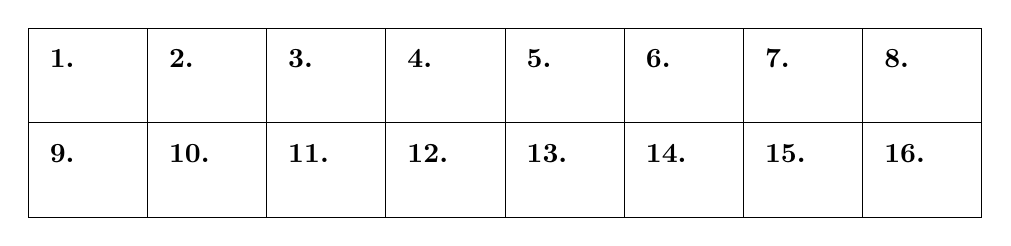
\begin{tikzpicture}
  % ---- 根据题数自动设置：16题为 8×2，20题为 10×2 ----
  \pgfmathtruncatemacro{\cols}{ifthenelse(\answerkeytotal<=16,8,10)}
  \pgfmathsetlengthmacro{\boxw}{(\linewidth-0.4pt)/\cols}
  \pgfmathsetlengthmacro{\boxh}{1.2cm}
  \pgfmathsetlengthmacro{\offset}{0.15cm}

  \foreach \num in {1,...,\answerkeytotal} {
    \pgfmathtruncatemacro{\row}{ifthenelse(\num<=\cols,0,1)}
    \pgfmathtruncatemacro{\col}{mod(\num-1,\cols)}
    \pgfmathsetlengthmacro{\x}{\col*\boxw}
    \pgfmathsetlengthmacro{\y}{-\row*\boxh}
    \draw (\x,\y) rectangle ++(\boxw,\boxh);
    \node[anchor=north west] at (\x+\offset,\y+\boxh-\offset) {\textbf{\num.}};
  }
\end{tikzpicture}

\end{flushleft}

\begin{question}
已知关于 $x$ 的不等式 $\dfrac{ax - 1}{x + 1} < 0$ 的解集为 $\{x \mid x < -1 \text{ 或 } x > -\dfrac{1}{2}\}$，则实数 $a$ 的值为： \paren[B]
    \begin{choices}
        \item $2$
        \item $-2$
        \item $\dfrac{1}{2}$
        \item $-\dfrac{1}{2}$
    \end{choices}
\end{question}
\begin{solution}
    由不等式 $\dfrac{ax-1}{x+1}<0$ 的解集反求实数 $a$。\\
    该分式不等式的两个分界点分别为 $x=-1$ 和 $x=\dfrac{1}{a}$，与已知解集比较即可确定 $a$。
    \begin{align*}
        \frac{1}{a} &= -\frac{1}{2} \\
        a &= -2
    \end{align*}
    故选 B。
\end{solution}

%region 范围：高中数学-分式不等式 | 考点：分式不等式的因式分解与符号分析法 | 难度：中等
\begin{question}
    解不等式 $\dfrac{2x^2-3x+1}{x^2+5x+6} \geq 0$ 。 \paren[A]
    \begin{choices}
        \item $x < -3$ 或 $-2 < x \leq \dfrac{1}{2}$ 或 $x \geq 1$
        \item $-3 < x < -2$ 或 $\dfrac{1}{2} < x < 1$
        \item $x \in \mathbb{R}$
        \item $x < -3$ 或 $-2 < x < \dfrac{1}{2}$ 或 $x > 1$
    \end{choices}
\end{question}

\begin{solution}
    求不等式 $\dfrac{2x^2-3x+1}{x^2+5x+6} \geq 0$ 的解集。\\
    先将分子分母因式分解，再用符号分析法确定各区间的正负。
    \begin{align*}
        \frac{2x^2-3x+1}{x^2+5x+6} &\geq 0 \\
        \frac{(2x-1)(x-1)}{(x+2)(x+3)} &\geq 0
    \end{align*}
    \[
        x < -3 \ \text{或} \ -2 < x \leq \frac{1}{2} \ \text{或} \ x \geq 1
    \]
    故选 A。
\end{solution}
%endregion


% \begin{question}已知关于 $x$ 的不等式 $ax^2+bx+c>0$ 的解集为 $(-1,2)$，则不等式 $cx^2-bx+a<0$ 的解集为： \paren[A]\begin{choices}
%     \item $\left(-\dfrac{1}{2},1\right)$
%     \item $\left(-\infty,-\dfrac{1}{2}\right)\cup(1,+\infty)$
%     \item $\left(-1,\dfrac{1}{2}\right)$
%     \item $(-\infty,-1)\cup\left(\dfrac{1}{2},+\infty\right)$
% \end{choices}
% \end{question}\begin{solution}\textbf{解析：}由不等式 $ax^2+bx+c>0$ 的解集为 $(-1,2)$ 可知：

% 1. $a<0$；
% 2. $x_1=-1$ 与 $x_2=2$ 是方程 $ax^2+bx+c=0$ 的两根。

% 由韦达定理得：
% \[
%     \begin{cases}
%         -1+2=-\dfrac{b}{a} \\
%         -1\times2=\dfrac{c}{a}
%     \end{cases}
%     \implies
%     \begin{cases}
%         b=-a \\
%         c=-2a
%     \end{cases}
% \]

% 将 $b,c$ 代入所求不等式 $cx^2-bx+a<0$：
% \[
%     -2ax^2+ax+a<0
% \]

% 因 $a<0$，两边同除以 $a$，不等号方向改变：
% \[
%     -2x^2+x+1>0
% \]
% 即：
% \[
%     2x^2-x-1<0
% \]

% 因式分解得：
% \[
%     (2x+1)(x-1)<0
% \]

% 解得 $-\dfrac{1}{2}<x<1$。

% 故选 A。
% \end{solution}

%region 范围：不等式 | 考点：分式不等式的解法与等价转化 | 难度：中等
\begin{question}
    已知实数 $x$ 满足分式不等式 $\displaystyle\frac{2x-1}{x+1} \ge 1$，则该不等式的解集为 \paren[C]
    \begin{choices}
        \item $\{x \mid x \ge 2\}$
        \item $\{x \mid x > -1\}$
        \item $\{x \mid x \ge 2 \text{ 或 } x < -1\}$
        \item $\{x \mid -1 < x \le 2\}$
    \end{choices}
\end{question}

\begin{solution}
    求分式不等式 $\dfrac{2x-1}{x+1} \ge 1$ 的解集。\\
    移项通分化为标准分式不等式形式，再转化为整式不等式组求解。
    \begin{align*}
        \frac{2x-1}{x+1} - 1 &\ge 0 \\
        \frac{(2x-1)-(x+1)}{x+1} &\ge 0 \\
        \frac{x-2}{x+1} &\ge 0
    \end{align*}
    \[
        \begin{cases} (x-2)(x+1) \ge 0 \\ x+1 \neq 0 \end{cases}
        \implies x \ge 2 \ \text{或} \ x < -1
    \]
    故选 C。
\end{solution}
%endregion

%region 范围：函数 | 考点：函数的定义与垂直线检验法（Vertical Line Test） | 难度：中等
\begin{question}
    在平面直角坐标系 $xOy$ 中，下列各图所示的曲线中，能表示 $y$ 是 $x$ 的函数的是 \paren[B]
    \begin{choices}
        \item 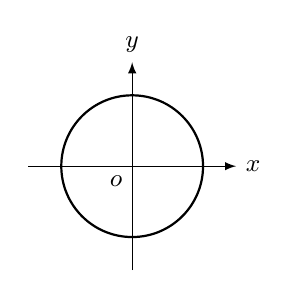
\begin{tikzpicture}[scale=0.6, baseline=(current bounding box.center)]
                \draw[-latex] (-2.2,0) -- (2.2,0) node[right] {\small $x$};
                \draw[-latex] (0,-2.2) -- (0,2.2) node[above] {\small $y$};
                \node[below left] at (0,0) {\small $o$};
                \draw[thick] (0,0) circle (1.5);
              \end{tikzpicture}
        \item 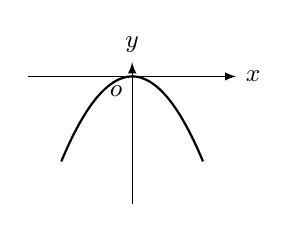
\begin{tikzpicture}[scale=0.6, baseline=(current bounding box.center)]
                \draw[-latex] (-2.2,2.2) -- (2.2,2.2) node[right] {\small $x$}; % 调整坐标轴位置适配抛物线
                \draw[-latex] (0,-0.5) -- (0,2.5) node[above] {\small $y$};
                \node[below left] at (0,2.2) {\small $o$};
                \draw[thick, domain=-1.5:1.5, samples=50, smooth] plot (\x, {2.2 - 0.8*\x*\x});
              \end{tikzpicture}
        \item \begin{tikzpicture}[scale=0.6, baseline=(current bounding box.center)]
                \draw[-latex] (-1,0) -- (2.5,0) node[right] {\small $x$};
                \draw[-latex] (0,-1.8) -- (0,1.8) node[above] {\small $y$};
                \node[below left] at (0,0) {\small $o$};
                \draw[thick, domain=-1.3:1.3, samples=50, smooth] plot ({1.2 + 0.5*\x*\x}, \x);
              \end{tikzpicture}
        \item 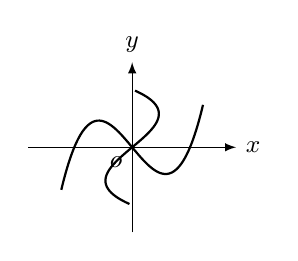
\begin{tikzpicture}[scale=0.6, baseline=(current bounding box.center)]
                \draw[-latex] (-2.2,0) -- (2.2,0) node[right] {\small $x$};
                \draw[-latex] (0,-1.8) -- (0,1.8) node[above] {\small $y$};
                \node[below left] at (0,0) {\small $o$};
                \draw[thick, domain=-1.5:1.5, samples=60, smooth] plot (\x, {0.8*\x*\x*\x - 1.2*\x});
                % 旋转或修改使其不满足函数定义（令其多值）
                \begin{scope}[rotate=90]
                \draw[thick, domain=-1.2:1.2, samples=60, smooth] plot (\x, {0.8*\x*\x*\x - 1.2*\x});
                \end{scope}
              \end{tikzpicture}
    \end{choices}
\end{question}

\begin{solution}
    判断四个图象中哪一个能表示 $y$ 是 $x$ 的函数。\\
    用垂直线检验法：任意竖直线与图象至多一个交点，才符合函数定义。
    \[
        \text{选项 B 为开口向下的抛物线，任意竖直线与其至多一个交点，满足函数定义}
    \]
    故选 B。
\end{solution}
%endregion

%region 范围：函数 | 考点：函数的概念与韦恩图（Venn diagram）表示法 | 难度：中等
\begin{question}
    设集合 $A = \{1, 2, 3\}$，集合 $B = \{a, b, c\}$，下列各范恩图（Venn）所示的对应关系 $f$ 中，能构成从集合 $A$ 到集合 $B$ 的函数的是 \paren[D]
    \begin{choices}
        \item 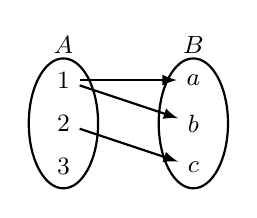
\begin{tikzpicture}[scale=0.55, baseline=(current bounding box.center)]
                % 集合 A
                \draw[thick] (0,0) ellipse (0.8cm and 1.5cm);
                \node at (0,1.8) {\small $A$};
                \node (A1) at (0,1) {\small 1};
                \node (A2) at (0,0) {\small 2};
                \node (A3) at (0,-1) {\small 3};
                % 集合 B
                \draw[thick] (3,0) ellipse (0.8cm and 1.5cm);
                \node at (3,1.8) {\small $B$};
                \node (B1) at (3,1) {\small $a$};
                \node (B2) at (3,0) {\small $b$};
                \node (B3) at (3,-1) {\small $c$};
                % 映射箭头
                \draw[-latex, thick] (A1) -- (B1);
                \draw[-latex, thick] (A1) -- (B2);
                \draw[-latex, thick] (A2) -- (B3);
              \end{tikzpicture}
        \item 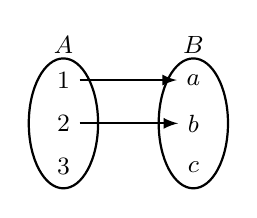
\begin{tikzpicture}[scale=0.55, baseline=(current bounding box.center)]
                % 集合 A
                \draw[thick] (0,0) ellipse (0.8cm and 1.5cm);
                \node at (0,1.8) {\small $A$};
                \node (A1) at (0,1) {\small 1};
                \node (A2) at (0,0) {\small 2};
                \node (A3) at (0,-1) {\small 3};
                % 集合 B
                \draw[thick] (3,0) ellipse (0.8cm and 1.5cm);
                \node at (3,1.8) {\small $B$};
                \node (B1) at (3,1) {\small $a$};
                \node (B2) at (3,0) {\small $b$};
                \node (B3) at (3,-1) {\small $c$};
                % 映射箭头
                \draw[-latex, thick] (A1) -- (B1);
                \draw[-latex, thick] (A2) -- (B2);
              \end{tikzpicture}
        \item 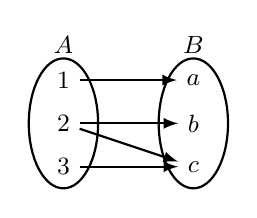
\begin{tikzpicture}[scale=0.55, baseline=(current bounding box.center)]
                % 集合 A
                \draw[thick] (0,0) ellipse (0.8cm and 1.5cm);
                \node at (0,1.8) {\small $A$};
                \node (A1) at (0,1) {\small 1};
                \node (A2) at (0,0) {\small 2};
                \node (A3) at (0,-1) {\small 3};
                % 集合 B
                \draw[thick] (3,0) ellipse (0.8cm and 1.5cm);
                \node at (3,1.8) {\small $B$};
                \node (B1) at (3,1) {\small $a$};
                \node (B2) at (3,0) {\small $b$};
                \node (B3) at (3,-1) {\small $c$};
                % 映射箭头
                \draw[-latex, thick] (A1) -- (B1);
                \draw[-latex, thick] (A2) -- (B2);
                \draw[-latex, thick] (A2) -- (B3);
                \draw[-latex, thick] (A3) -- (B3);
              \end{tikzpicture}
        \item 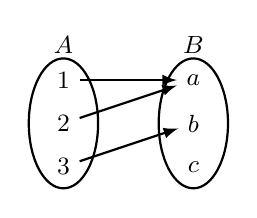
\begin{tikzpicture}[scale=0.55, baseline=(current bounding box.center)]
                % 集合 A
                \draw[thick] (0,0) ellipse (0.8cm and 1.5cm);
                \node at (0,1.8) {\small $A$};
                \node (A1) at (0,1) {\small 1};
                \node (A2) at (0,0) {\small 2};
                \node (A3) at (0,-1) {\small 3};
                % 集合 B
                \draw[thick] (3,0) ellipse (0.8cm and 1.5cm);
                \node at (3,1.8) {\small $B$};
                \node (B1) at (3,1) {\small $a$};
                \node (B2) at (3,0) {\small $b$};
                \node (B3) at (3,-1) {\small $c$};
                % 映射箭头
                \draw[-latex, thick] (A1) -- (B1);
                \draw[-latex, thick] (A2) -- (B1);
                \draw[-latex, thick] (A3) -- (B2);
              \end{tikzpicture}
    \end{choices}
\end{question}

\begin{solution}
    判断哪个韦恩图所示对应关系能构成从集合 $A$ 到集合 $B$ 的函数。\\
    函数须满足两点：$A$ 中每个元素都有对应元素（任意性），且对应元素唯一（唯一性）。
    \[
        \text{选项 D 中 } A \text{ 的每个元素都恰有一条箭头射出，同时满足任意性与唯一性}
    \]
    故选 D。
\end{solution}
%endregion

% %region 范围：函数 | 考点：分式、一元二次方程判别式法 | 难度：难
% \begin{question}
%     求函数 $\displaystyle f(x) = \frac{x^2 - x + 1}{x^2 + x + 1}$ 的值域。\paren[A]
%     \begin{choices}
%         \item $\displaystyle \left[ \frac{1}{3}, 3 \right]$
%         \item $\displaystyle \left( \frac{1}{3}, 3 \right)$
%         \item $\displaystyle \left( -\infty, \frac{1}{3} \right] \cup [3, +\infty)$
%         \item $\displaystyle \left[ -3, -\frac{1}{3} \right]$
%     \end{choices}
% \end{question}

% \begin{solution}
%     \textbf{解析：} \\
%     步骤 1：分析题意与知识点引入。\\
%     本题要求分式函数的值域。由于分子分母均为一元二次多项式，且定义域为 $x \in \mathbb{R}$（因为分母 $x^2 + x + 1 = (x + \frac{1}{2})^2 + \frac{3}{4} > 0$ 恒成立），最常用的解题策略是“反求法”或“一元二次方程判别式法”。令 $\displaystyle y = \frac{x^2 - x + 1}{x^2 + x + 1}$，将其转化为关于 $x$ 的一元二次方程。\\

%     步骤 2：公式计算与推导验证。\\
%     去分母并整理，可得：
%     \[ \displaystyle y(x^2 + x + 1) = x^2 - x + 1 \]
%     \[ \displaystyle (y - 1)x^2 + (y + 1)x + (y - 1) = 0 \]
    
%     分类讨论：
%     当 $y = 1$ 时，方程化为 $2x = 0$，解得 $x = 0$。即 $x=0$ 时，$y=1$，所以 $1$ 在值域内。
    
%     当 $y \neq 1$ 时，上述方程为关于 $x$ 的一元二次方程。由于 $x \in \mathbb{R}$，方程必须有实数根，故判别式 $\Delta \ge 0$。
%     \[ \displaystyle \Delta = (y + 1)^2 - 4(y - 1)^2 \ge 0 \]
%     展开并化简：
%     \[ \displaystyle y^2 + 2y + 1 - 4(y^2 - 2y + 1) \ge 0 \]
%     \[ \displaystyle -3y^2 + 10y - 3 \ge 0 \]
%     两边同乘 $-1$ 改变不等号方向：
%     \[ \displaystyle 3y^2 - 10y + 3 \le 0 \]
%     十字相乘因式分解：
%     \[ \displaystyle (3y - 1)(y - 3) \le 0 \]
%     解得：$\displaystyle \frac{1}{3} \le y \le 3$。
%     又因为当 $y=1$ 时也在此区间内，故所求值域为 $\displaystyle \left[ \frac{1}{3}, 3 \right]$。\\
    
%     以下为该函数的图像辅助理解，可明显看出其上下界：
%     \begin{center}
%     \begin{tikzpicture}[scale=1.2]
%         % 坐标轴
%         \draw[->] (-4,0) -- (4,0) node[right] {$x$};
%         \draw[->] (0,-0.5) -- (0,3.5) node[above] {$y$};
%         \node[below left] at (0,0) {$O$};
        
%         % 绘制函数曲线
%         \draw[smooth, samples=100, domain=-3.5:3.5, thick, blue] plot (\x, {(\x*\x - \x + 1)/(\x*\x + \x + 1)});
        
%         % 辅助线：最大值与最小值
%         \draw[dashed, red] (-4,3) -- (4,3) node[right] {$y=3$};
%         \draw[dashed, red] (-4,0.333) -- (4,0.333) node[right] {$y=\frac{1}{3}$};
        
%         % 极值点标注
%         \filldraw[black] (-1,3) circle (1.5pt) node[above left] {$(-1, 3)$};
%         \filldraw[black] (1,0.333) circle (1.5pt) node[below right] {$(1, \frac{1}{3})$};
%     \end{tikzpicture}
%     \end{center}
    
%     步骤 3：结论梳理与干扰项分析。\\
%     正确答案为 $\displaystyle \left[ \frac{1}{3}, 3 \right]$。\\
%     干扰项 B 错误，因为学生在求解 $\Delta \ge 0$ 时可能误写为严格大于号 $\Delta > 0$，忽略了等号（即函数能取到最值）；\\
%     干扰项 C 错误，这是解不等式 $-3y^2 + 10y - 3 \ge 0$ 时，未变号直接求两边区间导致的典型错误；\\
%     干扰项 D 错误，这是在分解因式 $(3y - 1)(y - 3)$ 时发生正负号混淆所致。\\
    
%     故选 A。
% \end{solution}
% %endregion


%region 范围：高中数学 - 函数 | 考点：分段函数逆向求值（已知函数值求自变量） | 难度：中等
\begin{question}
    设函数 $f(x)$ 定义为三段分段函数，其表达式为：
    $$f(x) = \begin{cases} x + 3, & x < 0 \\ x^2 - 1, & 0 \leq x < 2 \\ 2x - 1, & x \geq 2 \end{cases}$$
    若 $f(a) = 3$，求 $a$ 的值。 \paren[B]
    \begin{choices}
        \item $a = 0$
        \item $a = 2$
        \item $a = -2$
        \item $a = 4$
    \end{choices}
\end{question}

\begin{solution}
    已知分段函数 $f(x)$，$f(a)=3$，求 $a$ 的值。\\
    须逐段假设代入求解，并检验所得值是否落在该段的定义区间内。
    \begin{align*}
        x<0: \quad a+3 &= 3 \implies a=0 \ (\text{舍，不满足 } x<0) \\
        0\leq x<2: \quad a^2-1 &= 3 \implies a=\pm2 \ (\text{均舍，不满足区间}) \\
        x\geq2: \quad 2a-1 &= 3 \implies a=2 \ (\text{满足 } x\geq2)
    \end{align*}
    故选 B。
\end{solution}
%endregion

%region 范围：高中数学 - 函数的复合与待定系数法 | 考点：函数复合（f(f(x))）、待定系数法解方程组 | 难度：中等
\begin{question}
    已知函数 $f(x) = mx + n$（其中 $m, n$ 均为常数，且 $m > 0$），对任意实数 $x$ 恒有$f(f(x)) = 4x + 9$，求 $f(x)$ 。 \paren[C]
    \begin{choices}
        \item $f(x) = -2x - 9$
        \item $f(x) = 2x - 3$
        \item $f(x) = 2x + 3$
        \item $f(x) = 4x + 3$
    \end{choices}
\end{question}

\begin{solution}
    已知 $f(x)=mx+n$（$m>0$）且 $f(f(x))=4x+9$，求 $f(x)$。\\
    代入复合函数展开式，比较系数得关于 $m,n$ 的方程组。
    \begin{align*}
        f(f(x)) &= m(mx+n)+n = m^2x+(mn+n) \\
        m^2 &= 4, \quad n(m+1)=9
    \end{align*}
    \begin{align*}
        m &= 2 \ (m>0) \\
        n(2+1) &= 9 \implies n = 3
    \end{align*}
    故选 C。
\end{solution}
%endregion

%region 范围：高中数学 - 二次函数的图象与性质 | 考点：抛物线开口方向、顶点、与坐标轴交点的图象判断 | 难度：中等
\begin{question}
    已知二次函数 $y = x^2 -2x -3 $,
    下列哪一个图象正确地表示了该函数？ \paren[A]
    \begin{choices}
        \item
        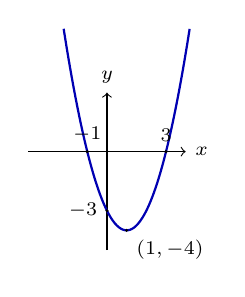
\begin{tikzpicture}[scale=0.25, baseline={(0,0)}]
            \draw[->] (-4,0) -- (4,0) node[right] {\scriptsize $x$};
            \draw[->] (0,-5) -- (0,3) node[above] {\scriptsize $y$};
            \draw[thick, blue!70!black, domain=-2.2:4.2, samples=60, smooth]
                plot (\x, {(\x)^2 - 2*\x - 3});
            \filldraw (1,-4) circle (1.3pt) node[below right, font=\scriptsize] {$(1,-4)$};
            \filldraw (-1,0) circle (1.3pt) node[above, font=\scriptsize] {$-1$};
            \filldraw (3,0) circle (1.3pt) node[above, font=\scriptsize] {$3$};
            \filldraw (0,-3) circle (1.3pt) node[left, font=\scriptsize] {$-3$};
        \end{tikzpicture}

        \item
        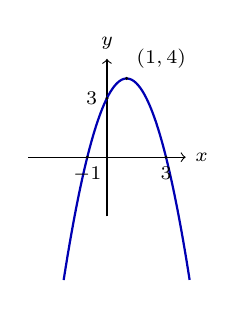
\begin{tikzpicture}[scale=0.25, baseline={(0,0)}]
            \draw[->] (-4,0) -- (4,0) node[right] {\scriptsize $x$};
            \draw[->] (0,-3) -- (0,5) node[above] {\scriptsize $y$};
            \draw[thick, blue!70!black, domain=-2.2:4.2, samples=60, smooth]
                plot (\x, {-((\x)^2 - 2*\x - 3)});
            \filldraw (1,4) circle (1.3pt) node[above right, font=\scriptsize] {$(1,4)$};
            \filldraw (-1,0) circle (1.3pt) node[below, font=\scriptsize] {$-1$};
            \filldraw (3,0) circle (1.3pt) node[below, font=\scriptsize] {$3$};
            \filldraw (0,3) circle (1.3pt) node[left, font=\scriptsize] {$3$};
        \end{tikzpicture}

        \item
        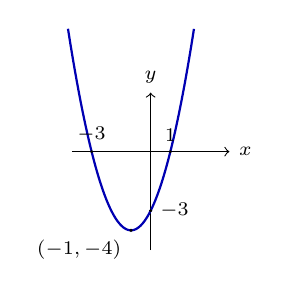
\begin{tikzpicture}[scale=0.25, baseline={(0,0)}]
            \draw[->] (-4,0) -- (4,0) node[right] {\scriptsize $x$};
            \draw[->] (0,-5) -- (0,3) node[above] {\scriptsize $y$};
            \draw[thick, blue!70!black, domain=-4.2:2.2, samples=60, smooth]
                plot (\x, {(\x)^2 + 2*\x - 3});
            \filldraw (-1,-4) circle (1.3pt) node[below left, font=\scriptsize] {$(-1,-4)$};
            \filldraw (-3,0) circle (1.3pt) node[above, font=\scriptsize] {$-3$};
            \filldraw (1,0) circle (1.3pt) node[above, font=\scriptsize] {$1$};
            \filldraw (0,-3) circle (1.3pt) node[right, font=\scriptsize] {$-3$};
        \end{tikzpicture}

        \item
        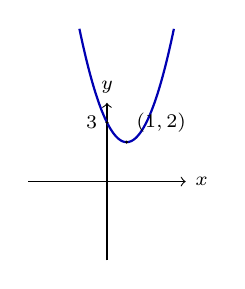
\begin{tikzpicture}[scale=0.25, baseline={(0,0)}]
            \draw[->] (-4,0) -- (4,0) node[right] {\scriptsize $x$};
            \draw[->] (0,-4) -- (0,4) node[above] {\scriptsize $y$};
            \draw[thick, blue!70!black, domain=-1.4:3.4, samples=60, smooth]
                plot (\x, {(\x)^2 - 2*\x + 3});
            \filldraw (1,2) circle (1.3pt) node[above right, font=\scriptsize] {$(1,2)$};
            \filldraw (0,3) circle (1.3pt) node[left, font=\scriptsize] {$3$};
        \end{tikzpicture}
    \end{choices}
\end{question}

\begin{solution}
    判断哪个图象正确表示二次函数 $y=x^2-2x-3$。\\
    由系数确定开口方向，再求顶点坐标与坐标轴交点。
    \begin{align*}
        a=1>0 &\implies \text{开口向上} \\
        x_0 = -\frac{b}{2a} &= -\frac{-2}{2} = 1, \quad y_0 = 1-2-3=-4 \\
        x^2-2x-3=0 &\implies (x-3)(x+1)=0 \implies x=-1,3
    \end{align*}
    \[
        \text{顶点 } (1,-4)\text{，与 } x \text{ 轴交于 } (-1,0),(3,0)\text{，与 } y \text{ 轴交于 } (0,-3)
    \]
    故选 A。
\end{solution}
%endregion


%region 范围：高中数学 - 反函数 | 考点：反函数的图象与原函数图象关于直线 y=x 对称 | 难度：中等
    \begin{question}
        已知函数 $y = (x-1)^2$，其定义域 $D_f = [1, +\infty)$，图象如图所示：

        \begin{center}
        \begin{tikzpicture}[scale=0.7]
            \draw[->] (-1,0) -- (4.5,0) node[right] {\scriptsize $x$};
            \draw[->] (0,-1) -- (0,4.5) node[above] {\scriptsize $y$};
            \node[below left] at (0,0) {\scriptsize $O$};
            \draw[thick, blue!70!black, domain=1:3, samples=60, smooth]
                plot (\x, {(\x-1)^2});
            \filldraw (1,0) circle (1.5pt) node[below, font=\scriptsize] {$(1,0)$};
            \filldraw (2,1) circle (1.5pt) node[right, font=\scriptsize] {$(2,1)$};
            \filldraw (3,4) circle (1.5pt) node[above, font=\scriptsize] {$(3,4)$};
        \end{tikzpicture}
        \end{center}

        下列哪一个图象是其反函数的图象？ \paren[B]
        \begin{choices}
            \item
            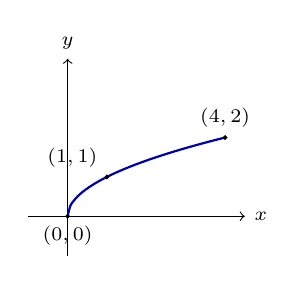
\begin{tikzpicture}[scale=0.5, baseline={(0,0)}]
                \draw[->] (-1,0) -- (4.5,0) node[right] {\scriptsize $x$};
                \draw[->] (0,-1) -- (0,4) node[above] {\scriptsize $y$};
                \draw[thick, blue!70!black, domain=0:4, samples=60, smooth]
                    plot (\x, {sqrt(\x)});
                \filldraw (0,0) circle (1.3pt) node[below, font=\scriptsize] {$(0,0)$};
                \filldraw (1,1) circle (1.3pt) node[above left, font=\scriptsize] {$(1,1)$};
                \filldraw (4,2) circle (1.3pt) node[above, font=\scriptsize] {$(4,2)$};
            \end{tikzpicture}

            \item
            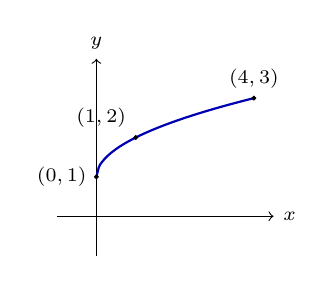
\begin{tikzpicture}[scale=0.5, baseline={(0,0)}]
                \draw[->] (-1,0) -- (4.5,0) node[right] {\scriptsize $x$};
                \draw[->] (0,-1) -- (0,4) node[above] {\scriptsize $y$};
                \draw[thick, blue!70!black, domain=0:4, samples=60, smooth]
                    plot (\x, {1+sqrt(\x)});
                \filldraw (0,1) circle (1.3pt) node[left, font=\scriptsize] {$(0,1)$};
                \filldraw (1,2) circle (1.3pt) node[above left, font=\scriptsize] {$(1,2)$};
                \filldraw (4,3) circle (1.3pt) node[above, font=\scriptsize] {$(4,3)$};
            \end{tikzpicture}

            \item
            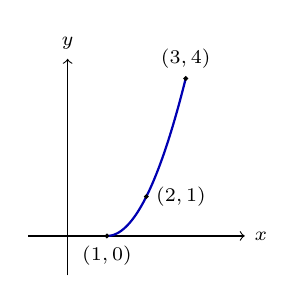
\begin{tikzpicture}[scale=0.5, baseline={(0,0)}]
                \draw[->] (-1,0) -- (4.5,0) node[right] {\scriptsize $x$};
                \draw[->] (0,-1) -- (0,4.5) node[above] {\scriptsize $y$};
                \draw[thick, blue!70!black, domain=1:3, samples=60, smooth]
                    plot (\x, {(\x-1)^2});
                \filldraw (1,0) circle (1.3pt) node[below, font=\scriptsize] {$(1,0)$};
                \filldraw (2,1) circle (1.3pt) node[right, font=\scriptsize] {$(2,1)$};
                \filldraw (3,4) circle (1.3pt) node[above, font=\scriptsize] {$(3,4)$};
            \end{tikzpicture}

            \item
            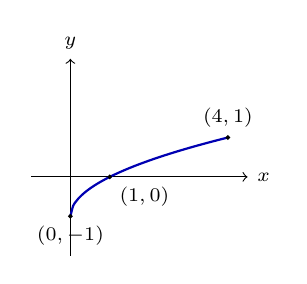
\begin{tikzpicture}[scale=0.5, baseline={(0,0)}]
                \draw[->] (-1,0) -- (4.5,0) node[right] {\scriptsize $x$};
                \draw[->] (0,-2) -- (0,3) node[above] {\scriptsize $y$};
                \draw[thick, blue!70!black, domain=0:4, samples=60, smooth]
                    plot (\x, {-1+sqrt(\x)});
                \filldraw (0,-1) circle (1.3pt) node[below, font=\scriptsize] {$(0,-1)$};
                \filldraw (1,0) circle (1.3pt) node[below right, font=\scriptsize] {$(1,0)$};
                \filldraw (4,1) circle (1.3pt) node[above, font=\scriptsize] {$(4,1)$};
            \end{tikzpicture}
        \end{choices}
    \end{question}

\begin{solution}
    已知 $y=(x-1)^2$，$D_f=[1,+\infty)$，求其反函数的图象。\\
    互换 $x,y$ 后解出 $y$，再依原函数值域确定取舍符号。
    \begin{align*}
        x &= (y-1)^2 \\
        y-1 &= \pm\sqrt{x} \\
        y &= 1+\sqrt{x} \ (\text{取正号，因反函数值域 } y\geq1)
    \end{align*}
    故选 B。
\end{solution}
%endregion

\newpage

%region 范围：高中数学 - 二元一次不等式组表示的平面区域 | 考点：不等式组的整理（移项、变号）与区域图象判断 | 难度：困难
\begin{question}
    在平面直角坐标系中，下列不等式组所表示的平面区域（阴影部分）是哪一个图象？
    $$\begin{cases} 4 \geq x + y \\ y - x \geq -2 \\ x + 1 \geq 0 \end{cases}$$
    \paren[A]
    \begin{choices}
        \item
        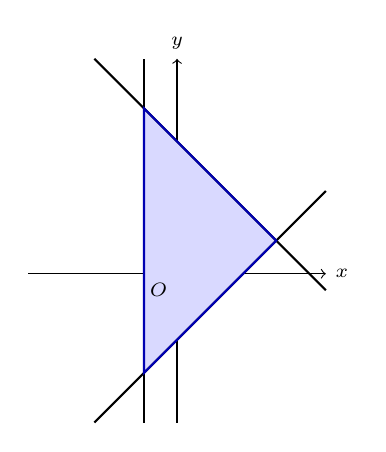
\begin{tikzpicture}[scale=0.42, baseline={(0,1)}]
            \draw[->] (-4.5,0) -- (4.5,0) node[right] {\scriptsize $x$};
            \draw[->] (0,-4.5) -- (0,6.5) node[above] {\scriptsize $y$};
            \fill[blue!15] (-1,-3) -- (3,1) -- (-1,5) -- cycle;
            \draw[thick] (-2.5,6.5) -- (4.5,-0.5); % 直线 x+y=4
            \draw[thick] (-2.5,-4.5) -- (4.5,2.5); % 直线 y-x=-2
            \draw[thick] (-1,-4.5) -- (-1,6.5);    % 直线 x=-1
            \draw[thick, blue!70!black] (-1,-3) -- (3,1) -- (-1,5) -- cycle;
            \node[below left] at (0,0) {\scriptsize $O$};
        \end{tikzpicture}

        \item
        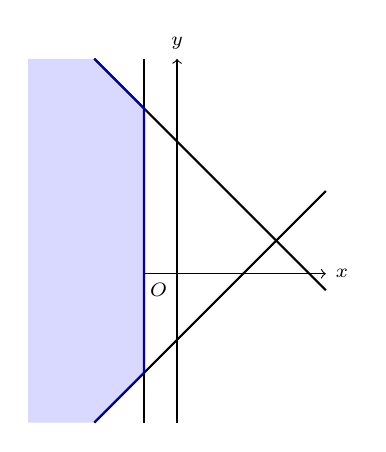
\begin{tikzpicture}[scale=0.42, baseline={(0,1)}]
            \draw[->] (-4.5,0) -- (4.5,0) node[right] {\scriptsize $x$};
            \draw[->] (0,-4.5) -- (0,6.5) node[above] {\scriptsize $y$};
            \fill[blue!15] (-4.5,-4.5) -- (-2.5,-4.5) -- (-1,-3) -- (-1,5) -- (-2.5,6.5) -- (-4.5,6.5) -- cycle;
            \draw[thick] (-2.5,6.5) -- (4.5,-0.5);
            \draw[thick] (-2.5,-4.5) -- (4.5,2.5);
            \draw[thick] (-1,-4.5) -- (-1,6.5);
            \draw[thick, blue!70!black] (-2.5,-4.5) -- (-1,-3) -- (-1,5) -- (-2.5,6.5);
            \node[below left] at (0,0) {\scriptsize $O$};
        \end{tikzpicture}

        \item
        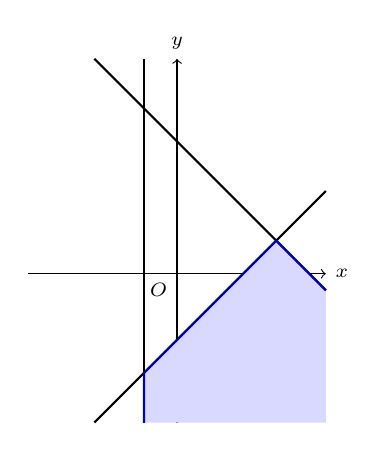
\begin{tikzpicture}[scale=0.42, baseline={(0,1)}]
            \draw[->] (-4.5,0) -- (4.5,0) node[right] {\scriptsize $x$};
            \draw[->] (0,-4.5) -- (0,6.5) node[above] {\scriptsize $y$};
            \fill[blue!15] (-1,-4.5) -- (4.5,-4.5) -- (4.5,-0.5) -- (3,1) -- (-1,-3) -- cycle;
            \draw[thick] (-2.5,6.5) -- (4.5,-0.5);
            \draw[thick] (-2.5,-4.5) -- (4.5,2.5);
            \draw[thick] (-1,-4.5) -- (-1,6.5);
            \draw[thick, blue!70!black] (-1,-4.5) -- (-1,-3) -- (3,1) -- (4.5,-0.5);
            \node[below left] at (0,0) {\scriptsize $O$};
        \end{tikzpicture}

        \item
        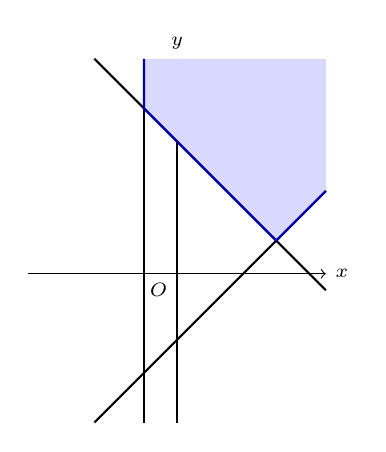
\begin{tikzpicture}[scale=0.42, baseline={(0,1)}]
            \draw[->] (-4.5,0) -- (4.5,0) node[right] {\scriptsize $x$};
            \draw[->] (0,-4.5) -- (0,6.5) node[above] {\scriptsize $y$};
            \fill[blue!15] (-1,6.5) -- (-1,5) -- (3,1) -- (4.5,2.5) -- (4.5,6.5) -- cycle;
            \draw[thick] (-2.5,6.5) -- (4.5,-0.5);
            \draw[thick] (-2.5,-4.5) -- (4.5,2.5);
            \draw[thick] (-1,-4.5) -- (-1,6.5);
            \draw[thick, blue!70!black] (-1,6.5) -- (-1,5) -- (3,1) -- (4.5,2.5);
            \node[below left] at (0,0) {\scriptsize $O$};
        \end{tikzpicture}
    \end{choices}
\end{question}

\begin{solution}
    判断不等式组 $\begin{cases}4\geq x+y\\y-x\geq-2\\x+1\geq0\end{cases}$ 所表示的平面区域图象。\\
    先将各不等式整理为标准形式，求出边界交点，再用原点检验区域取舍。
    \begin{align*}
        x+y &\leq 4, \quad y \geq x-2, \quad x \geq -1 \\
        x+y=4 \ \cap \ y=x-2 &\implies (3,1) \\
        y=x-2 \ \cap \ x=-1 &\implies (-1,-3) \\
        x+y=4 \ \cap \ x=-1 &\implies (-1,5)
    \end{align*}
    \[
        (0,0): 0\leq4 \checkmark,\ 0\geq-2 \checkmark,\ 1\geq0 \checkmark \implies \text{原点在区域内}
    \]
    故选 A。
\end{solution}
%endregion

% 范围：高中数学 - 函数与复合函数 | 考点：换元法求函数解析式（识别已按 g(x) 分解的表达式结构） | 难度：中等
\begin{question}
    已知函数 $g(x) = x + 1$，且$f\big(g(x)\big) = \big(x+1\big)^2 - 3\big(x+1\big) + 5$，求 $f(x)$ 。 \paren[D]
    \begin{choices}
        \item $f(x) = x^2 + 3x + 5$
        \item $f(x) = x^2 - x + 3$
        \item $f(x) = x^2 - 3x + 3$
        \item $f(x) = x^2 - 3x + 5$
    \end{choices}
\end{question}

\begin{solution}
    已知 $g(x)=x+1$，$f(g(x))=(x+1)^2-3(x+1)+5$，求 $f(x)$。\\
    右边表达式已完整保留 $g(x)=x+1$ 整体结构，设 $t=x+1$ 直接代换即可。
    \begin{align*}
        f(t) &= t^2-3t+5 \\
        f(x) &= x^2-3x+5
    \end{align*}
    故选 D。
\end{solution}

\newpage
%region 范围：函数与图像 | 考点：幂函数、反比例函数图像特征识别（$1/x$、$\sqrt{x}$、$x^2$、$1/x^2$） | 难度：中等
\begin{question}
    观察下列甲、乙、丙、丁四个函数图像，判断下列选项中，函数与图像的配对完全正确的是 \paren[A]

    \begin{center}
    \begin{tabular}{cccc}
    \begin{tikzpicture}[scale=0.55]
        \draw[->] (-2.3,0) -- (2.3,0) node[right] {\scriptsize $x$};
        \draw[->] (0,-2.3) -- (0,2.3) node[above] {\scriptsize $y$};
        \draw[domain=0.3:2.2, samples=40, smooth, thick] plot (\x, {1/\x});
        \draw[domain=-2.2:-0.3, samples=40, smooth, thick] plot (\x, {1/\x});
    \end{tikzpicture}
    &
    \begin{tikzpicture}[scale=0.55]
        \draw[->] (-2.3,0) -- (2.3,0) node[right] {\scriptsize $x$};
        \draw[->] (0,-2.3) -- (0,2.3) node[above] {\scriptsize $y$};
        \draw[domain=0:2, samples=40, smooth, thick] plot (\x, {sqrt(\x)});
    \end{tikzpicture}
    &
    \begin{tikzpicture}[scale=0.55]
        \draw[->] (-2.3,0) -- (2.3,0) node[right] {\scriptsize $x$};
        \draw[->] (0,-2.3) -- (0,2.3) node[above] {\scriptsize $y$};
        \draw[domain=-1.5:1.5, samples=40, smooth, thick] plot (\x, {\x*\x});
    \end{tikzpicture}
    &
    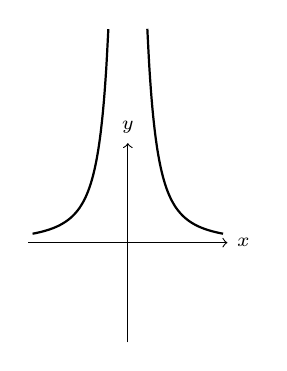
\begin{tikzpicture}[scale=0.55]
        \draw[->] (-2.3,0) -- (2.3,0) node[right] {\scriptsize $x$};
        \draw[->] (0,-2.3) -- (0,2.3) node[above] {\scriptsize $y$};
        \draw[domain=0.45:2.2, samples=40, smooth, thick] plot (\x, {1/(\x*\x)});
        \draw[domain=-2.2:-0.45, samples=40, smooth, thick] plot (\x, {1/(\x*\x)});
    \end{tikzpicture}
    \\
    甲 & 乙 & 丙 & 丁
    \end{tabular}
    \end{center}

    \begin{choices}
        \item 甲：$\displaystyle y=\frac{1}{x}$；乙：$y=\sqrt{x}$；丙：$y=x^2$；丁：$\displaystyle y=\frac{1}{x^2}$
        \item 甲：$\displaystyle y=\frac{1}{x^2}$；乙：$y=\sqrt{x}$；丙：$y=x^2$；丁：$\displaystyle y=\frac{1}{x}$
        \item 甲：$\displaystyle y=\frac{1}{x}$；乙：$y=x^2$；丙：$y=\sqrt{x}$；丁：$\displaystyle y=\frac{1}{x^2}$
        \item 甲：$\displaystyle y=\frac{1}{x^2}$；乙：$y=x^2$；丙：$y=\sqrt{x}$；丁：$\displaystyle y=\frac{1}{x}$
    \end{choices}
\end{question}

\begin{solution}
    判断甲乙丙丁四个图像与函数的正确配对。\\
    依各函数的定义域、奇偶性及所在象限逐一辨识图像特征。
    \[
        \text{甲：} y=\frac{1}{x}\text{（原点对称，一三象限）；\ 乙：} y=\sqrt{x}\text{（第一象限，增长趋缓）}
    \]
    \[
        \text{丙：} y=x^2\text{（$y$ 轴对称，开口向上）；\ 丁：} y=\frac{1}{x^2}\text{（$y$ 轴对称，一二象限）}
    \]
    故选 A。
\end{solution}
%endregion



% 范围：高中数学 - 函数的值域 | 考点：分式函数值域的求法（反解法／排除法） | 难度：基础
\begin{question}
    求函数 $f(x) = \dfrac{1}{x+2}$ 的值域。 \paren[C]
    \begin{choices}
        \item $R_f = \mathbb{R}$
        \item $R_f = \{y \mid y \neq -2\}$
        \item $R_f = \{y \mid y \neq 0\}$
        \item $R_f = (0, +\infty)$
    \end{choices}
\end{question}

\begin{solution}
    求函数 $f(x)=\dfrac{1}{x+2}$ 的值域。\\
    用反解法：设 $y=f(x)$，将 $x$ 用 $y$ 表示，再依 $x$ 有解的条件反推 $y$ 的范围。
    \begin{align*}
        y &= \frac{1}{x+2} \\
        x &= \frac{1}{y} - 2
    \end{align*}
    \[
        \text{须 } y\neq0\text{（否则 } \tfrac{1}{y} \text{ 无意义），故值域为 } \{y\mid y\neq0\}
    \]
    故选 C。
\end{solution}



% 范围：高中数学 - 角度与弧度、扇形的弧长与面积公式 | 考点：扇形周长与面积的综合应用 | 难度：中等
\begin{question}
    用一根长度为 $100\text{cm}$ 的铁丝弯折成一个半径为 $35\text{cm}$ 的扇形。求该扇形的面积。

    \begin{center}
    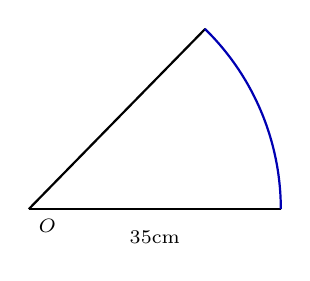
\begin{tikzpicture}[scale=1.6]
        \coordinate (O) at (0,0);
        \coordinate (A) at (2,0);
        \coordinate (B) at (1.4,1.43);
        \draw[thick] (O) -- (A);
        \draw[thick] (O) -- (B);
        \draw[thick, blue!70!black] (A) arc (0:45.7:2);
        \node[below right, font=\scriptsize] at (O) {$O$};
        \node[below, font=\scriptsize] at (1,-0.1) {$35\text{cm}$};
        % \node[above, font=\scriptsize] at (1,1.15) {$35\text{cm}$};
    \end{tikzpicture}
    \end{center}
    \paren[C]
    \begin{choices}
        \item $525\text{cm}^2$
        \item $1050\text{cm}^2$
        \item $1137.5\text{cm}^2$
        \item $1750\text{cm}^2$
    \end{choices}
\end{question}

\begin{solution}
    用长 $100\text{cm}$ 的铁丝弯成半径 $35\text{cm}$ 的扇形，求其面积。\\
    设弧长为 $l$，扇形周长由两条半径与弧长构成，再代入面积公式 $S=\frac{1}{2}lr$。
    \begin{align*}
        2(35) + l &= 100 \implies l = 30 \\
        S &= \frac{1}{2} \times 30 \times 35 = 525
    \end{align*}
    故选 C。
\end{solution}

% 范围：高中数学 - 角度与弧度的互化 | 考点：角度制与弧度制的转换公式及常见混淆点 | 难度：基础
\begin{question}
    下列关于角度与弧度互化的说法，正确的是： \paren[B]
    \begin{choices}
        \item $1$ 弧度 $= 180°$
        \item $300° = \dfrac{5\pi}{3}$ 弧度
        \item 把角度化为弧度时，应将角度数乘以 $\dfrac{180}{\pi}$
        \item $-\dfrac{2\pi}{3}$ 弧度 $= -150°$
    \end{choices}
\end{question}

\begin{solution}
    判断关于角度与弧度互化的说法哪个正确。\\
    核心公式为 $\pi$ 弧度 $=180°$，角度化弧度乘以 $\frac{\pi}{180}$。
    \[
        300° \times \frac{\pi}{180} = \frac{300\pi}{180} = \frac{5\pi}{3}
    \]
    故选 B。
\end{solution}


% 范围：高中数学 - 弧度制下扇形的弧长与面积公式 | 考点：由弧度与弧长求扇形面积（公式 $l=r\theta$，$S=\frac{1}{2}lr$） | 难度：中等

\begin{question}
    已知一扇形的圆心角为 $\dfrac{2\pi}{3}$ 弧度，弧长为 $4\pi\text{cm}$，求该扇形的面积。

    \begin{center}
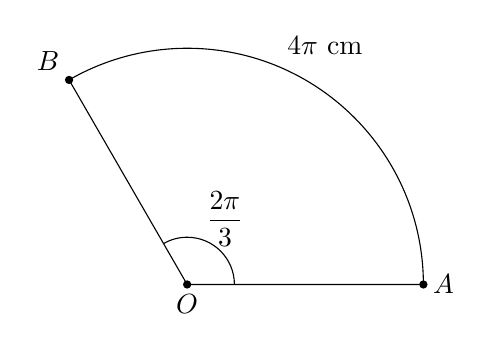
\begin{tikzpicture}[scale=1]\coordinate (O) at (0,0);\coordinate (A) at (3,0);\coordinate (B) at (120:3);\draw (O) -- (A) arc (0:120:3) -- cycle;\fill (O) circle (1.5pt) node[below] {$O$};\fill (A) circle (1.5pt) node[right] {$A$};\fill (B) circle (1.5pt) node[above left] {$B$};\pic[draw,"$\dfrac{2\pi}{3}$",angle radius=6mm,angle eccentricity=1.6]{angle=A--O--B};\node at (60:3.5) {$4\pi\text{ cm}$};\end{tikzpicture}
    \end{center}
    \paren[C]
    \begin{choices}
        \item $24\pi \ \text{cm}^2$
        \item $\dfrac{\pi}{3} \ \text{cm}^2$
        \item $12\pi \ \text{cm}^2$
        \item $\dfrac{4\pi^2}{3} \ \text{cm}^2$
    \end{choices}
\end{question}

\begin{solution}
    已知扇形圆心角 $\dfrac{2\pi}{3}$ 弧度，弧长 $4\pi\text{cm}$，求扇形面积。\\
    先由弧长公式 $l=r\theta$ 求半径，再代入扇形面积公式 $S=\frac{1}{2}lr$。
    \begin{align*}
        r &= \frac{l}{\theta} = \frac{4\pi}{\frac{2\pi}{3}} = 6 \\
        S &= \frac{1}{2} \times 4\pi \times 6 = 12\pi
    \end{align*}
    故选 C。
\end{solution}



\vfill % 与上方内容保持距离

\noindent
\newlength{\sigwidth}
\settowidth{\sigwidth}{（\hspace{4em}师）}

\begin{tabular*}{\textwidth}{@{\extracolsep{\fill}} l l l}
    出题： & 审题： & 审核： \\[4em]
    \rule{\sigwidth}{0.5pt} &
    \rule{\sigwidth}{0.5pt} &
    \rule{\sigwidth}{0.5pt} \\
    （\hspace{0em} \setterteacher ） &
    （\hspace{0em} \reviewteacher ） &
    （\hspace{0em} \auditteacher ） \\
\end{tabular*}


\newpage
\begin{center}
\textbf{参考答案}

\begin{tikzpicture}
  \pgfmathtruncatemacro{\cols}{ifthenelse(\answerkeytotal<=16,8,10)}
  \pgfmathsetlengthmacro{\boxw}{(\linewidth-0.4pt)/\cols}
  \pgfmathsetlengthmacro{\boxh}{1.2cm}
  \pgfmathsetlengthmacro{\offset}{0.15cm}

  \answerkeyitems
\end{tikzpicture}
\end{center}
\end{document}